\documentclass[12pt]{article}
\usepackage{fullpage,enumitem,amsmath,amssymb,graphicx}
\DeclareMathOperator{\E}{\mathbb{E}}

\begin{document}

\begin{center}
{\Large CS 236 Fall 2019 Homework [2]}

\begin{tabular}{rl}
SUNet ID: & [zyuan84] \\
Name: & [Zheng Yuan] \\
\end{tabular}
\end{center}

By turning in this assignment, I agree by the Stanford honor code and declare
that all of this is my own work.

\section*{Problem 1}
\begin{enumerate}
	\item 
	see the code
	
	\item 
	see the code
	
	\item 
	python run\_vae.py: Table. \ref{table:vae}
	
	\begin{table}[ht]
		\caption{run vae experiments} % title of Table
		\centering % used for centering table
		\begin{tabular}{c c c c} % centered columns (4 columns)
			\hline\hline %inserts double horizontal lines
			run ID & negative ELBO & KL term & reconstruction loss \\ [0.5ex] % inserts table
			%heading
			\hline % inserts single horizontal line
			1 & 101.4059 & 19.3038 & 82.1021 \\ % inserting body of the table
			2 & 101.5392 & 19.1540 & 82.3852 \\
			3 & 101.7680 & 19.5879 & 82.1801 \\
			4 & 100.6686 & 19.0667 & 81.6018 \\
			5 & 101.8012 & 19.4861 & 82.3150 \\ 
			mean & 101.4366 & 19.3197 & 82.1168 \\
			std & 0.4594 & 0.2187 & 0.3085 \\[1ex] % [1ex] adds vertical space
			\hline %inserts single line
		\end{tabular}
		\label{table:vae} % is used to refer this table in the text
	\end{table}

\item 200 digits sampled: Fig. \ref{fig:vae}
\begin{figure}
	\advance\leftskip-4cm
	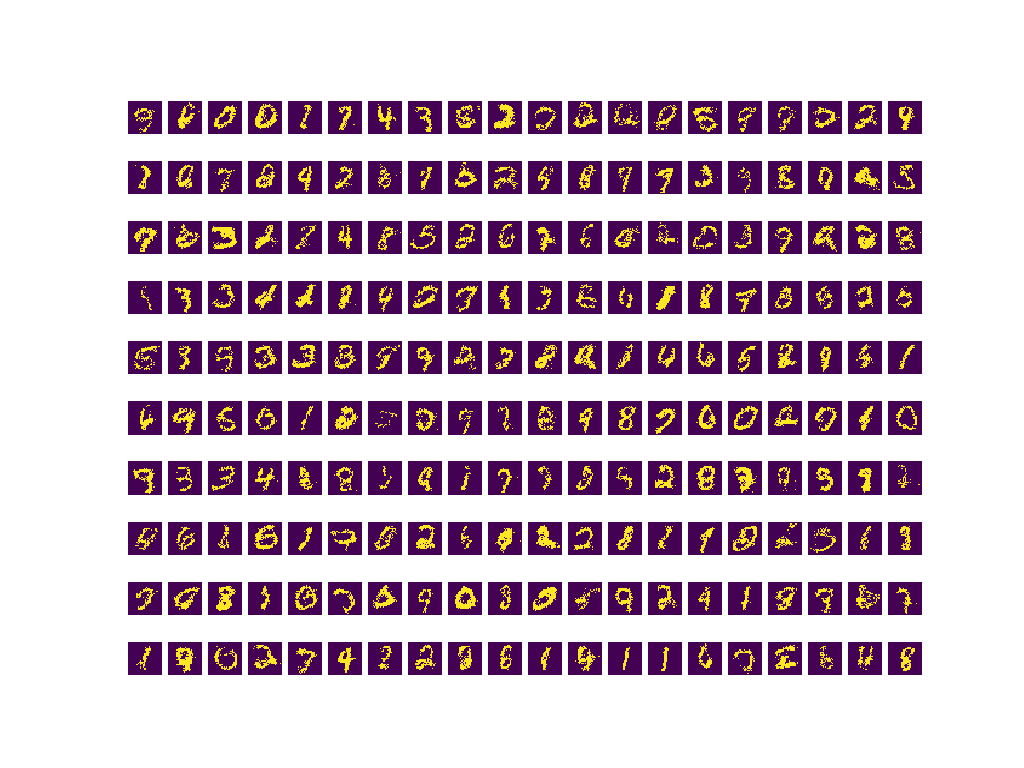
\includegraphics[scale=1.5]{vae.png}
	\caption{sampled by vae}

	\label{fig:vae}
\end{figure}
\end{enumerate}

\section*{Problem 2}

\begin{enumerate}
	\item 
	see the code
	
	\item 
	python run\_gmvae.py: Table. \ref{table:gmvae}
	
	\begin{table}[ht]
		\label{table:gmvae}
		\caption{run gmvae experiments} % title of Table
		\centering % used for centering table
		\begin{tabular}{c c c c} % centered columns (4 columns)
			\hline\hline %inserts double horizontal lines
			run ID & negative ELBO & KL term & reconstruction loss \\ [0.5ex] % inserts table
			%heading
			\hline % inserts single horizontal line
			1 & 98.7112 & 17.8145 & 80.8967 \\ % inserting body of the table
			2 & 99.7082 & 17.3642 & 82.3439 \\
			3 & 98.8653 &17.8933 & 80.9719 \\
			4 & 99.2312 & 18.0453 & 81.1859 \\
			5 & 99.0813 & 17.8141 &  81.2671 \\ 
			mean & 99.1194 & 17.7863 & 81.3331 \\
			std & 0.3847 & 0.2541 & 0.5849 \\[1ex] % [1ex] adds vertical space
			\hline %inserts single line
		\end{tabular}
		\label{table:gmvae} % is used to refer this table in the text
	\end{table}
	
	\item 200 digits sampled: Fig. \ref{fig:gmvae}
	\begin{figure}
		\advance\leftskip-4cm
		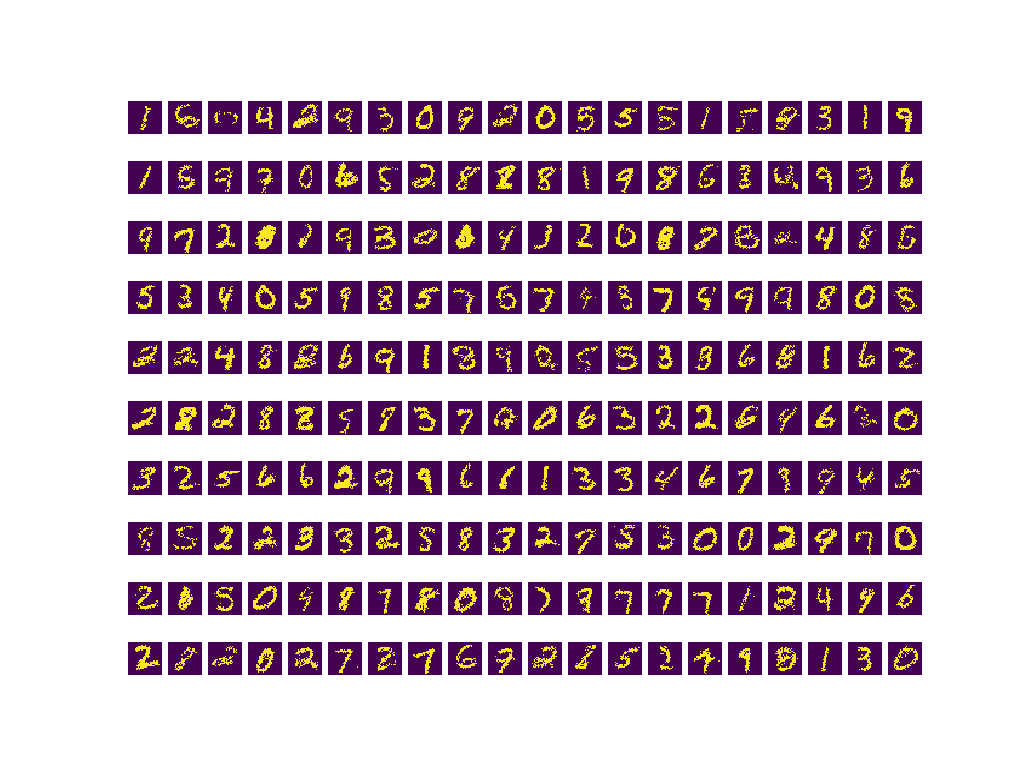
\includegraphics[scale=1.5]{gmvae.png}
		\caption{sampled by gmvae}
		\label{fig:gmvae}
	\end{figure}
\end{enumerate}

\section*{Problem 3}
\begin{enumerate}
	\item 
	Proof
	
	\begin{equation}
	\begin{split}
	\mathcal{L}_m(x; \theta, \phi) =& \mathbb{E}_{z^{(1)}, \ldots, z^{(m)} \overset{\text{i.i.d.}}{\sim} q_\phi(z|x)} \left(\log \frac{1}{m} \sum_{i=1}^m \frac{p_\theta(x,z^{(i)})}{q_\phi(z^{(i)}|x)} \right) \\
	<=& \log \mathbb{E}_{z^{(1)}, \ldots, z^{(m)} \overset{\text{i.i.d.}}{\sim} q_\phi(z|x)} \left( \frac{1}{m} \sum_{i=1}^m \frac{p_\theta(x,z^{(i)})}{q_\phi(z^{(i)}|x)} \right) \\
	=& \log  \frac{1}{m}  \sum_{i=1}^m \mathbb{E}_{z^{(1)},\ldots, z^{(m)} \overset{\text{i.i.d.}}{\sim} q_\phi(z|x)} \left( \frac{p_\theta(x,z^{(i)})}{q_\phi(z^{(i)}|x)} \right) \\
	=& \log  \frac{1}{m}  \sum_{i=1}^m \mathbb{E}_{z {\sim} q_\phi(z|x)} \left( \frac{p_\theta(x,z)}{q_\phi(z|x)} \right) \\
	=& \log  \mathbb{E}_{z {\sim} q_\phi(z|x)} \left( \frac{p_\theta(x,z)}{q_\phi(z|x)} \right) \\
	=& \log  \int q_\phi(z|x)  \frac{p_\theta(x,z)}{q_\phi(z|x)} dz \\	
	=& \log p_\theta(x)
	\end{split}
	\end{equation}
	
	\begin{equation}
	\begin{split}
	\mathcal{L}_m(x; \theta, \phi) =& \mathbb{E}_{z^{(1)}, \ldots, z^{(m)} \overset{\text{i.i.d.}}{\sim} q_\phi(z|x)} \left(\log \frac{1}{m} \sum_{i=1}^m \frac{p_\theta(x,z^{(i)})}{q_\phi(z^{(i)}|x)} \right) \\
	>=& \mathbb{E}_{z^{(1)}, \ldots, z^{(m)} \overset{\text{i.i.d.}}{\sim} q_\phi(z|x)} \left( \frac{1}{m} \sum_{i=1}^m \log \frac{p_\theta(x,z^{(i)})}{q_\phi(z^{(i)}|x)} \right)  \\
	=& \frac{1}{m} \sum_{i=1}^m  \mathbb{E}_{z^{(1)}, \ldots, z^{(m)} \overset{\text{i.i.d.}}{\sim} q_\phi(z|x)} \left(  \log \frac{p_\theta(x,z^{(i)})}{q_\phi(z^{(i)}|x)} \right) \\
	=&  \mathbb{E}_{z \overset{\text{i.i.d.}}{\sim} q_\phi(z|x)} \left(  \log \frac{p_\theta(x,z)}{q_\phi(z|x)} \right) \\
	&= \mathcal{L}_1(x; \theta, \phi)
	\end{split}
\end{equation}

\item 
see the code

\item 
python run\_vae.py --train 0

NELBO: 101.4059066772461. KL: 19.303831100463867. Rec: 82.10210418701172 \\
Negative IWAE-1: 101.423583984375 \\
Negative IWAE-10: 98.38631439208984 \\
Negative IWAE-100: 97.94550323486328 \\
Negative IWAE-1000: 97.9181137084961 \\

\item
python run\_gmvae.py --train 0

NELBO: 98.71127319335938. KL: 17.814559936523438. Rec: 80.89671325683594 \\
Negative IWAE-1: 98.66850280761719 \\
Negative IWAE-10: 96.22054290771484 \\
Negative IWAE-100: 95.39800262451172 \\
Negative IWAE-1000: 94.81982421875 \\
	
	
\end{enumerate}

\section*{Problem 4}
\begin{enumerate}
	\item 
	Test set classification accuracy: supervised 0.7609999775886536
	
	\item 
	see the code
	
	\item 
	Test set classification accuracy: semi supervised 0.918999969959259
\end{enumerate}


\section*{Problem 5}

\begin{enumerate}
	\item 
	\begin{equation}
	\begin{split}
	\log p_\theta(x | y) =& \log \int p_{\theta}(x|y, z) p_{\theta}(z|y) dz \\
	=& \log \int p_{\theta} (x, z|y) dz \\
	=& \log \mathbb{E}_{z {\sim} q_\phi(z|x, y)}  \frac{p_{\theta} (x, z|y)}{q_{\phi}(z|x, y)} \\
	>=& \mathbb{E}_{z {\sim} q_\phi(z|x, y)}   \log \frac{p_{\theta} (x, z|y)}{q_{\phi}(z|x, y)}  \\
	=& \mathrm{ELBO}(x; \theta, \phi, y) \\
	\end{split}
	\end{equation}	
	
	\item Fig. \ref{fig:fsvae}
	
	\begin{figure}
		\advance\leftskip-4cm
		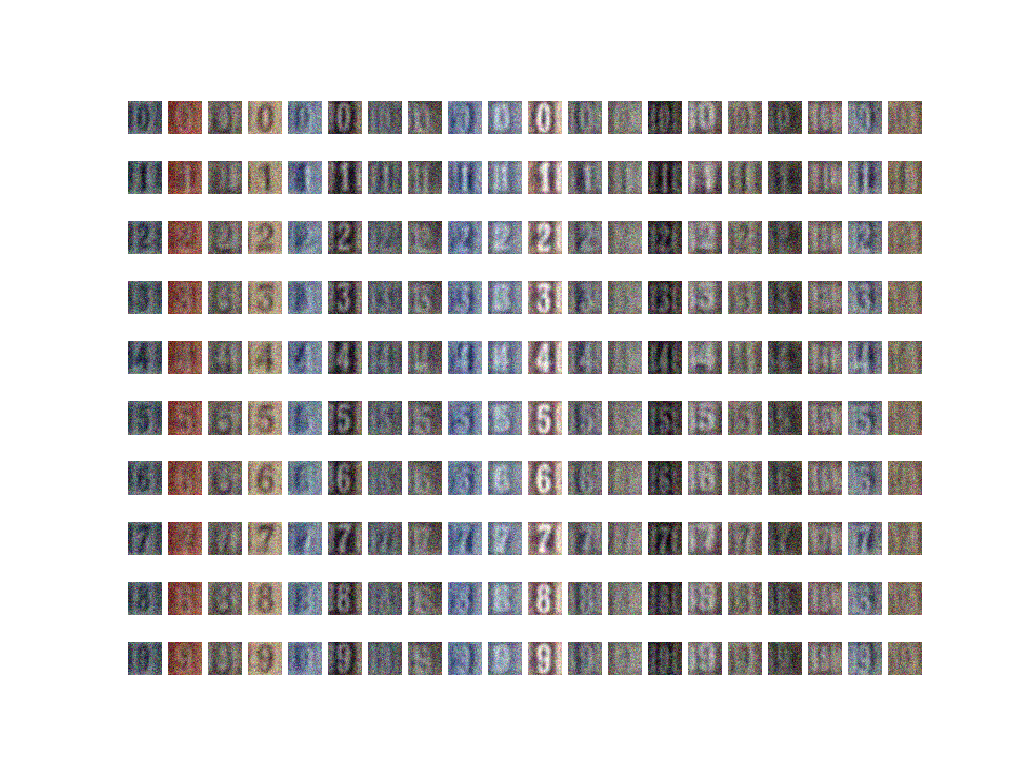
\includegraphics[scale=1.5]{fsvae.png}
		\caption{sampled by fsvae}
		\label{fig:fsvae}
	\end{figure}	

	
\end{enumerate}

\end{document}